\ProvidesFile{rutitlepage.dtx}[2022/02/21 v3.0 Radboud University Titlepage]
\documentclass{ltxdoc}
\newcommand{\messagespace}{\text{$\mathcal{M}$}}
\newcommand{\messageinstance}{\text{$m$}}
\newcommand{\ciphertextspace}{\text{$\mathcal{C}$}}
\newcommand{\ciphertextinstance}{\text{$c$}}
\newcommand{\associateddataspace}{\text{$\mathcal{A}$}}
\newcommand{\associateddatainstance}{\text{$a$}}
\newcommand{\tagspace}{\text{$\mathcal{T}$}}
\newcommand{\taginstance}{\text{$t$}}
\newcommand{\keyspace}{\text{$\mathcal{K}$}}
\newcommand{\keyinstance}{\text{$k$}}
\newcommand{\noncespace}{\text{$\mathcal{N}$}}
\newcommand{\nonceinstance}{\text{$n$}}
\newcommand{\lockspace}{\text{$\mathcal{L}$}}
\newcommand{\lockinstance}{\text{$l$}}
\newcommand{\users}{\text{$N$}}
\newcommand{\user}{\text{$j$}}
\newcommand{\adversary}{\text{$A$}}
\newcommand{\sample}{\text{$\leftarrow$}}
\newcommand{\result}{\text{$\leftarrow$}}
\newcommand{\concatinate}{\text{$\|$}}

\newcommand{\advantage}[2]{\textbf{Adv}$_{\text{#1}}^{\text{#2}}$ }
\newcommand{\probabilityblock}[4]{\text{$|\text{Pr}[\text{#1}_{\text{#2}}^{\text{#3}}] - \text{Pr}[\text{#1}_{\text{#2}}^{\text{#4}}]|$}}

\newcommand{\pkc}{\text{Hybrid Encryption in a Multi-user Setting, revised}}
\newcommand{\gcrec}{\text{Generic Composition Reconsidered}}

\newcommand{\x}{\text{x}}
\usepackage{a4wide}
\usepackage{float}
\usepackage{graphicx}
\usepackage{array}
\usepackage[utf8]{inputenc}
\usepackage{rutitlepage}
\usepackage{fancyhdr}
\usepackage[style=ieee]{biblatex}
\usepackage[operators]{cryptocode}
\usepackage{amssymb}
\addbibresource{cryptobib/crypto.bib}
\GetFileInfo{rutitlepage.dtx}

\pagestyle{fancy}
\fancyhf{}
\lhead{Bachelor Thesis}
\rhead{Page \thepage}

\title{research proposal}
\author{stijnvandenput }
\date{20 May 2022}

\begin{document}
\maketitleru[
    layout=traditional,
    authors={Stijn Vandenput},
    authorstext={Author:},
    nextpagenr={-1},
    date={20/05/2022},
    institution={Radboud Honours Academy},
    others={Supervisors:}{Martijn Stam\\Bart Mennink},
    course={Bachelor Thesis},
    title={TBD}]

\section*{Abstract}

\pagenumbering{roman}
\newpage
\tableofcontents

\newpage
\pagenumbering{arabic}

\section{Introduction}
should consist of:
\begin{itemize}
	\item explaining the challenge
	\item my contribution
\end{itemize}
Within the field of cryptography there are a two different fields, symmetric and asymmetric crypto. The former is about situations where the users have a shared secret already, the latter is about situations where this is not the case. Sometimes work in asymmetric crypto uses constructions that are more common in symmetric crypto, and in this fashion, a paper by Giacon, Kiltz and Poettering \cite{PKC:GiaKilPoe18}, which we henceforth call \pkc{}, uses a construction that is very similar to Authenticated Encryption following the generic encrypt-then-MAC construction from Bellare and Namprempre \cite{AC:BelNam00}. This construction has since been revised in a paper by Namprempre1, Rogaway and Thomas Shrimpton \cite{EC:NamRogShr14}, which we henceforth call \gcrec{}, to be better applicable to common use cases. The aim of this thesis is to apply the knowledge of \gcrec{} to the setting of \pkc{} and in doing so, create a primitive for authenticated encryption in a asymmetric crypto setting.

\section{Preliminaries}
should consist of:
\begin{itemize}
    \item general notation
    \item AE
	\item PKE schemes
	\item nonces vs locks (and different iv's)
	\item game based security notions
\end{itemize}

\subsection{notation table}
Below is a table which highlights the differences in notation between \pkc and \gcrec, as well as give the notation I will be using.\\
\begin{tabular}{|c | c | c | c | m{5cm}|}
    \hline
    Name   &   \pkc   &   \gcrec   &   my notation & rough meaning \\[0.5 ex]
    \hline
    \hline
    message space   &   $\mathcal{M}$   &   $\mathcal{M}$   &   \messagespace & set of all possible message options \\
    \hline
    message   &   $m$   &   $M$   &   \messageinstance &  message the user sends \\
    \hline
    ciphertext space   &   $\mathcal{C}$   &   -   &   \ciphertextspace & set of all possible ciphertext options \\
    \hline
    ciphertext   &   $c$   &   $C$   &   \ciphertextinstance & encrypted message \\
    \hline
    associated data space   &   -   &   $\mathcal{A}$   &   \associateddataspace & set of all possible associated data options \\
    \hline
    associated data   &   -   &   $A$   &   \associateddatainstance & data you want to authenticate but not encrypt \\
    \hline
    tag space   &   $\mathcal{C}$   &   $\mathcal{T}$   &   \tagspace & set off all possible tag options \\
    \hline
    tag   &   $c$   &   $T$   &   \taginstance & output of mac function \\
    \hline
    key space   &   $\mathcal{K}$   &   $\mathcal{K}$   &   \keyspace & set of all possible key options \\
    \hline
    key   &   $k$   &   $K$   &   \keyinstance   & user key \\
    \hline
    nonce space   &   -   &   $\mathcal{N}$   &   \noncespace & set of all nonce options \\
    \hline
    nonce   &   -   &   $n$   &   \nonceinstance & number only used once \\
    \hline
    lock space   &   $\mathcal{T}$   &   -   &   \lockspace & set of all possible lock options \\
    \hline
    lock   &   $t$   &   -   &   \lockinstance & nonce that is bound to the user \\
    \hline
    users   &   $N$   &   -   &   \users & number of users \\
    \hline
    adversary   &   A   &   $\mathcal{A}$   &   \adversary & the bad guy \\
    \hline
    random sampling   &   $\leftarrow^{\$}$    &   $\twoheadleftarrow$   &   \sample & get a random ellermetn form the set \\
    \hline
    result of randomised function   &   $\leftarrow^{\$}$   &   -   &   \result & get the result of a randomised function with given inputs \\
    \hline
    result of function   &   $\leftarrow$   &   $\leftarrow$   &   \result & get the result of a function with given inputs \\
    \hline
    concatination   &   a$\|$b   &   a$\|$b   &   a\concatinate{}b & concatanation of two strings \\
    \hline
    true   &   \ensuremath{\mathit{true}}   &   -   &   \codetrue & boolean true \\
    \hline
    false   &   \ensuremath{\mathit{false}}   &   -   &   \codefalse & boolean false \\
    \hline
    invalid   &   $\bot$   &   $\bot$   &   \invalid & operation is invalid \\
    \hline
    %Name   &   \pkc   &   \GCrec   &   my notation & rough meaning \\
    %\hline
\end{tabular}\\
strings are binary and bit-wise

\section{Existing AE/DEM notations in more detail}
should consist of:
\begin{itemize}
	\item the definition of the two paper, if possible already brought more toward one notation standard
	\item explain how both relate to the preliminaries and overall story
\end{itemize}

\subsection{Existing notation from \pkc}
Below are the security notations from \pkc{} that are relevent for this thesis. Some of the variable names are rewritten towards a common notation with \gcrec.
\subsubsection{notation}
\messagespace{} is a message space, \keyspace{} is a finite key space, \lockspace{} is a lock space and \ciphertextspace{} is a ciphertext space. \users{} is the number of users.

\subsubsection{used primitives}
\begin{itemize}
    \item ADEM: the ADEM exists of tuple $(\text{A.enc}, \text{A.dec})$, A.enc is a deterministic algorithm that takes a key \keyinstance{} in \keyspace{}, a lock \lockinstance{} in \lockspace{} and a message \messageinstance{} in \messagespace{} and outputs a ciphertext \ciphertextinstance{} in \ciphertextspace{}. A.dec is a deterministic algorithm that takes a \keyinstance{} in \keyspace{}, a lock \lockinstance{} in \lockspace{} and a ciphertext \ciphertextinstance{} in \ciphertextspace{} and outputs a message \messageinstance{} in \messagespace{} or \invalid{} to indicate rejection. The correctness requirement is that for every combination of \keyinstance{}, \lockinstance{} and \messageinstance{} we have A.dec$(\keyinstance,\lockinstance,\text{A.enc}(\keyinstance,\lockinstance,\messageinstance))$ = \messageinstance. The security of the ADEM is defined with \advantage{ADEM,\adversary,\users}{l-miot-ind} = \probabilityblock{L-MIOT-IND}{\adversary,\users}{0}{1}, defined by the following game:
    \begin{figure}[H]
        \centering
        \begin{pchstack}[boxed,center,space=0.5cm]
            \pseudocode[lnstart=-1,linenumbering,head={\textbf{Game} L-MIOT-IND$^{b}_{\adversary,\users}$ }]{
            L \result \emptyset\\
            \pcfor \user \in [1..N]:\\
            \t \keyinstance_\user \sample \keyspace\\
            \t C_\user \result \emptyset\\
            b' \result \adversary\\
            \pcreturn b'
            }
            \pseudocode[lnstart=5,linenumbering,head={\textbf{Oracle} Oenc$(\user,\lockinstance,\messageinstance_0,\messageinstance_1)$}]{
                \pcif C_\user \neq \emptyset: \pcreturn \invalid\\
                \pcif \lockinstance \in L: \pcreturn \invalid\\
                L \result L \cup \{\lockinstance\}\\
                \lockinstance_\user \result \lockinstance\\
                \ciphertextinstance \result \text{A.enc}(\keyinstance_\user,\lockinstance_\user,\messageinstance_b)\\
                C_\user \result C_\user \cup \{\ciphertextinstance\}\\
                \pcreturn \ciphertextinstance
            }
            \pseudocode[lnstart=12,linenumbering,head={\textbf{Oracle} Odec(\user,\ciphertextinstance)}]{
                \pcif C_\user = \emptyset: \pcreturn \invalid\\
                \pcif \ciphertextinstance \in C_\user: \pcreturn \invalid\\
                \messageinstance \result \text{A.dec}(\keyinstance_\user,\lockinstance_\user,\ciphertextinstance)\\
                \pcreturn \messageinstance
            }
        \end{pchstack}
        \caption{L-MIOT-IND game, \adversary{} has access to oracles Oenc and Odec and the locks in line 10 and 15 are the same. The corresponding game can be found in \pkc{} figure 9.}
    \end{figure}
    
    \item AMAC: the AMAC exists of tuple $(\text{M.mac},\text{M.vrf})$. M.mac is a deterministic algorithm that takes a key \keyinstance{} in \keyspace{}, a lock \lockinstance{} in \lockspace{}, and a message \messageinstance{} in \messagespace{} and outputs a ciphertext \ciphertextinstance{} in \ciphertextspace{}. M.vrf takes a key \keyinstance{} in \keyspace{}, a lock \lockinstance{} in \lockspace{}, a message \messageinstance{} in \messagespace{} and a ciphertext \ciphertextinstance{} in \ciphertextspace{} and returns either \codetrue{} or \codefalse. The correctness requirement is that for every combination of \keyinstance{}, \lockinstance{} and \messageinstance{}, all corresponding \ciphertextinstance{} \result M.mac$(\keyinstance,\lockinstance,\messageinstance)$ gives M.vrf$(\keyinstance,\lockinstance,\messageinstance,\ciphertextinstance)$ = \codetrue. The security of the AMAC is defined with \advantage{AMAC,\adversary,\users}{L-MIOT-UF} = $\text{Pr}[\text{L-MIOT-UF}_{\adversary,\users}]$, defined by the following game:
    \begin{figure}[H]
        \centering
        \begin{pchstack}[boxed,center,space=0.5cm]
            \pseudocode[lnstart=-1,linenumbering,head={\textbf{Game} L-MIOT-UF$_{\adversary,\users}$ }]{
            \text{forged} \result 0\\
            L \result \emptyset\\
            \pcfor \user \in [1..N]:\\
            \t \keyinstance_\user \sample \keyspace\\
            \t T_\user \result \emptyset\\
            \textbf{run } \adversary\\
            \pcreturn \text{forged}
            }
            \pseudocode[lnstart=6,linenumbering,head={\textbf{Oracle} Omac$(\user,\lockinstance,\messageinstance)$}]{
                \pcif T_\user \neq \emptyset: \pcreturn \invalid\\
                \pcif \lockinstance \in L: \pcreturn \invalid\\
                L \result L \cup \{\lockinstance\}\\
                \lockinstance_\user \result \lockinstance\\
                \taginstance \result \text{M.mac}(\keyinstance_\user,\lockinstance_\user,\messageinstance)\\
                T_\user \result T_\user \cup \{(\messageinstance,\taginstance)\}\\
                \pcreturn \taginstance
            }
            \pseudocode[lnstart=13,linenumbering,head={\textbf{Oracle} Ovrf$(\user,\messageinstance,\taginstance)$}]{
                \pcif T_\user = \emptyset: \pcreturn \invalid\\
                \pcif (\messageinstance,\taginstance) \in T_\user: \pcreturn \invalid\\
                \pcif \text{M.vrf}(\keyinstance_\user,\lockinstance_\user,\messageinstance,\taginstance): \\
                \t \text{forged} \result 1\\
                \t \pcreturn \codetrue\\
                \pcelse : \pcreturn \codefalse
            }
        \end{pchstack}
        \caption{L-MIOT-UF game, \adversary{} has access to oracles Omac and Ovrf and the locks in line 11 and 16 are the same. The corresponding game can be found in \pkc{} figure 15.}
    \end{figure}
\end{itemize}

\subsubsection{goal}
The goal is to make a scheme ADEM' exists of tuple $(\text{A.enc'},\text{A.dec'})$ which has the same security of the ADEM, but is also secure against active attacks.

\subsubsection{Security model}
The security of the ADEM is defined with \advantage{ADEM',\adversary,\users}{l-miot-ind} = \probabilityblock{L-MIOT-IND}{\adversary,\users}{0}{1} where game L-MIOT-IND uses newly defined (A.enc',A.dec') instead of the former (A.enc,A.dec)

\subsubsection{construction}
The goal is met by creating new A.enc' and A.dec' calls which are build using the calls the primitives provide us:
\begin{figure}[H]
    \centering
    \begin{pchstack}[boxed,center,space=0.5cm]
        \pseudocode[lnstart=-1,linenumbering,head={\textbf{Proc} A.enc'$(\keyinstance,\lockinstance,\messageinstance)$}]{
        (\keyinstance_{dem},\keyinstance_{mac}) \result \keyinstance\\
        \ciphertextinstance' \result \text{A.enc}(\keyinstance_{dem},\lockinstance,\messageinstance)\\
        \taginstance \result \text{M.mac}(\keyinstance_{mac},\lockinstance,\ciphertextinstance')\\
        \ciphertextinstance \result (\ciphertextinstance',\taginstance)\\
        \pcreturn \ciphertextinstance
        }
        \pseudocode[lnstart=4,linenumbering,head={\textbf{Proc} A.dec'$(\keyinstance,\lockinstance,\ciphertextinstance)$}]{
            (\keyinstance_{dem},\keyinstance_{mac}) \result \keyinstance\\
            (\ciphertextinstance',\taginstance) \result \ciphertextinstance\\
            \pcif \text{M.vrf}(\keyinstance_{mac},\lockinstance,\ciphertextinstance',\taginstance):\\
            \t \messageinstance \result \text{A.dec}(\keyinstance_{dem},\lockinstance,\ciphertextinstance')\\
            \t \pcreturn \messageinstance\\
            \pcelse : \pcreturn \invalid
        }
    \end{pchstack}
    \caption{A.enc' and A.dec' calls, The corresponding calls can be found in \pkc{} figure 16.}
\end{figure}
\noindent The construction is deemed secure as for any \users{} and a \adversary{} that makes $Q_d$ many Odec queries, the exist $B$ and $C$ such that \advantage{ADEM',$A$,\users}{l-miot-ind} $\leq$ 2\advantage{AMAC,$B$,\users}{l-miot-uf} + \advantage{ADAM,$C$,\users}{l-miot-ind} holds. Where the running time of $B$ is at most that of $A$ plus the time required to run \users-many ADEM encapsulations and $Q_d$-many ADEM decapsulations and the running time of $C$ is the same as the running time of $A$. Additionally, $B$ poses at most $Q_d$-many Ovrf queries, and $C$ poses no Odec query.

\subsection{Existing notation from \gcrec}
Below are the security notations from \gcrec{} that are relevent for this thesis. Some of the variable names are rewritten towards a common notation with \pkc.
\subsubsection{notation}
\keyspace{} is a nonempty key space, \noncespace{} is a non-empty nonce space, \messagespace{} is a message space and \associateddataspace{} is the associated-data space. \messagespace{} contains at least two strings, and if \messagespace{} and \associateddataspace{} contain a string of length x, they must contain all strings of length x.

\subsubsection{used primitives}
    \begin{itemize}
        \item nE: A nonce-based encryption scheme is defined by triple $\mathit{\Pi}$ = $(\keyspace{},\text{E},\text{D})$. E is a deterministic encryption algorithm that takes three inputs $(\keyinstance,\nonceinstance,\messageinstance)$ to a value \ciphertextinstance, the length of \ciphertextinstance{} only depends the length of \keyinstance, \nonceinstance{} and \messageinstance. When $(\keyinstance,\nonceinstance,\messageinstance)$ is not in $\keyspace \times \noncespace \times \messagespace$, \ciphertextinstance{} will be \invalid. D is the decryption algorithm that takes three inputs $(\keyinstance,\nonceinstance,\ciphertextinstance)$ to a value \messageinstance. E and D are inverse of each other implying correctness (if E$(\keyinstance,\nonceinstance,\messageinstance)$ $= \ciphertextinstance \neq \invalid$, then D$(\keyinstance,\nonceinstance,\ciphertextinstance)$ = \messageinstance) and tidiness (if D$(\keyinstance,\nonceinstance,\ciphertextinstance)$ $= \messageinstance \neq \invalid$, then E$(\keyinstance,\nonceinstance,
        \messageinstance)$ = \ciphertextinstance). The security is defined as \advantage{$\mathit{\Pi}$,\adversary}{nE} = \probabilityblock{nE-IND\$}{\adversary}{0}{1}, where nE-IND\$ is defined as follows:
        \begin{figure}[H]
            \centering
            \begin{pchstack}[boxed,center,space=0.5cm]
                \pseudocode[lnstart=-1,linenumbering,head={\textbf{Game} nE-IND\$$^{b}_{\adversary}$ }]{
                    U = \emptyset\\
                    \keyinstance \sample \keyspace\\
                    b' \result \adversary\\
                    \pcreturn b'
                }
                \pseudocode[lnstart=4,linenumbering,head={\textbf{Oracle} Oenc$(\nonceinstance,\messageinstance)$}]{
                    \pcif \nonceinstance \in U : \pcreturn \invalid\\
                    U = U \cup \nonceinstance\\
                    \ciphertextinstance \result \text{E}(\keyinstance,\nonceinstance,\messageinstance)\\
                    \pcif b = 1 \wedge \ciphertextinstance \neq \invalid: \\
                    \t \ciphertextinstance \sample \{0,1\}^{\abs{\ciphertextinstance}}\\
                    \pcreturn \ciphertextinstance
                }
            \end{pchstack}
            \caption{nE-IND\$ game, \adversary{} has access to oracle Oenc and $U$ is the set of used nonces}
        \end{figure}
    
    
        \item MAC: The MAC is a deterministic algorithm F that takes in a \keyinstance{} in \keyspace{} and a string \messageinstance{} and outputs either a n-bit length \taginstance{} or \invalid. The domain of F is the set X such that F$(\keyinstance,\messageinstance)\neq \invalid$. The security is defined as \advantage{F,\adversary}{MAC} = \probabilityblock{MAC-PRF}{\adversary}{0}{1}, where MAC-PRF is defined as follows:
        \begin{figure}[H]
            \centering
            \begin{pchstack}[boxed,center,space=0.5cm]
                \pseudocode[lnstart=-1,linenumbering,head={\textbf{Game} MAC-PRF$^{b}_{\adversary}$ }]{
                    U = \emptyset\\
                    \keyinstance \sample \keyspace\\
                    b' \result \adversary\\
                    \pcreturn b'
                }
                \pseudocode[lnstart=3,linenumbering,head={\textbf{Oracle} Omac(\messageinstance)}]{
                    \pcif \messageinstance \in U : \pcreturn \invalid\\
                    U = U \cup \messageinstance\\
                    \taginstance \result \text{F}(\keyinstance,\messageinstance)\\
                    \pcif b = 1 \wedge \taginstance \neq \invalid: \\
                    \t \taginstance \sample \{0,1\}^{\abs{\taginstance}}\\
                    \pcreturn \taginstance
                }
            \end{pchstack}
            \caption{MAC-PRF, \adversary{} has access to oracle Omac and $U$ is the set of used messages}
        \end{figure}
    \end{itemize}

\subsubsection{goal}
The goal is a nonce-based authenticated encryption scheme defined by triple $\mathit{\Pi}$ = $(\keyspace{},\text{E},\text{D})$. E is a deterministic encryption algorithm that takes four inputs $(\keyinstance,\nonceinstance,\associateddatainstance,\messageinstance)$ to a value \ciphertextinstance, the length of \ciphertextinstance{} only depends the length of \keyinstance, \nonceinstance, \associateddatainstance{} and \messageinstance. When $(\keyinstance,\nonceinstance,\associateddatainstance,\messageinstance)$ is not in $\keyspace \times \noncespace \times \associateddataspace \times \messagespace$, \ciphertextinstance{} will be \invalid. D is the decryption algorithm that takes four inputs $(\keyinstance,\nonceinstance,\associateddatainstance,\ciphertextinstance)$ to a value \messageinstance. E and D are inverse of each other implying correctness (if E$(\keyinstance,\nonceinstance,\associateddatainstance,\messageinstance)$ $= \ciphertextinstance \neq \invalid$, then D$(\keyinstance,\nonceinstance,\associateddatainstance,\ciphertextinstance)$ = \messageinstance) and tidiness (if D$(\keyinstance,\nonceinstance,\associateddatainstance,\ciphertextinstance)$ $= \messageinstance \neq \invalid$, then E$(\keyinstance,\nonceinstance,\associateddatainstance,\messageinstance)$ = \ciphertextinstance)

\subsubsection{Security model}
The security is defined as \advantage{$\mathit{\Pi}$,\adversary}{nAE} = \probabilityblock{nAE-IND\$}{\adversary}{0}{1}, where nAE-IND\$ is defined as follows:
    \begin{figure}[H]
        \centering
        \begin{pchstack}[boxed,center,space=0.5cm]
            \pseudocode[lnstart=-1,linenumbering,head={\textbf{Game} nAE-IND\$$^{b}_{\adversary}$ }]{
                U = \emptyset\\
                Q = \emptyset\\
                \keyinstance \sample \keyspace\\
                b' \result \adversary\\
                \pcreturn b'
            }
            \pseudocode[lnstart=5,linenumbering,head={\textbf{Oracle} Oenc$(\nonceinstance,\associateddatainstance,\messageinstance)$}]{
                \pcif \nonceinstance \in U : \pcreturn \invalid\\
                U = U \cup \nonceinstance\\
                \pcif (\nonceinstance,\associateddatainstance,\messageinstance,\_) \in Q : \pcreturn \invalid\\
                \ciphertextinstance \result \text{E}(\keyinstance,\nonceinstance,\associateddatainstance,\messageinstance)\\
                \pcif b = 1 \wedge \ciphertextinstance \neq \invalid: \\
                \t \ciphertextinstance \sample \{0,1\}^{\abs{\ciphertextinstance}}\\
                Q = Q \cup (\nonceinstance,\associateddatainstance,\messageinstance,\ciphertextinstance)\\
                \pcreturn \ciphertextinstance
            }
            \pseudocode[lnstart=13,linenumbering,head={\textbf{Oracle} Odec$(\nonceinstance,\associateddatainstance,\ciphertextinstance)$}]{
                \pcif b = 1 : \pcreturn \bot\\
                \pcif (\nonceinstance,\associateddatainstance,\_,\ciphertextinstance) \in Q : \pcreturn \invalid\\
                \messageinstance \result \text{D} (\keyinstance,\nonceinstance,\associateddatainstance,\ciphertextinstance)\\
                Q = Q \cup (\nonceinstance,\associateddatainstance,\messageinstance,\ciphertextinstance)\\
                \pcreturn \messageinstance
            }
        \end{pchstack}
        \caption{nAE-IND\$ game, \adversary{} has access to oracles Oenc and Odec, $U$ is the set of used nonces and $Q$ is the set of query results. \_ denotes a variable that is irrelevant}
    \end{figure}

\subsubsection{construction}
The goal is met by creating different schemes that combine the mac and nE into a nAE.
We define the constructions secure as there is a tight reduction from breaking the nAE-security of the scheme to breaking the nE-security and the PRF security of the underlying primitives. Three different schemes, named N1, N2 and N3 were proven to be secure the can be viewed in \gcrec{} figure 6.

\section{New Definition}
should consist of:
\begin{itemize}
	\item syntax of the primitive (input, output, correctness, tidiness, expected bounds)
	\item game based code
	\item explanation of the choices made
	\item formal comparison with other choices
\end{itemize}

\subsection{notation}
\keyspace{} is a non-empty key space, \lockspace{} is a non-empty lock space and \messagespace{} is a message space. \messagespace{} contains at least two strings, and if it contains a string of length x, it must contain all strings of length x. \users{} is the number of users.

\subsection{goal}
The end goal is to build a lock-based one time use Authenticated Encryption scheme (loAE). The AE scheme is defined by tuple $(\text{AE.enc},\text{AE.dec})$. AE.enc is a deterministic encryption algorithm that takes three inputs $(\keyinstance,\lockinstance,\messageinstance)$ to a value \ciphertextinstance, the length of \ciphertextinstance{} only depends on the length of \keyinstance, \lockinstance{} and \messageinstance. When $(\keyinstance,\lockinstance,\messageinstance)$ is not in $\keyspace \times \lockspace \times \messagespace$, \ciphertextinstance{} will be \invalid. AE.dec is the decryption algorithm that takes three inputs $(\keyinstance,n,\ciphertextinstance)$ to a value \messageinstance. AE.enc and EA.dec are inverse of each other implying correctness (if AE.enc$(\keyinstance,\lockinstance,\messageinstance)$ $= \ciphertextinstance \neq \invalid$, then AE.dec$(\keyinstance,\lockinstance,\ciphertextinstance)$ = \messageinstance) and tidiness (if AE.dec$(\keyinstance,\lockinstance,\ciphertextinstance)$ $= \messageinstance \neq \invalid$, then AE.enc$(\keyinstance,\lockinstance,\messageinstance)$ = \ciphertextinstance).

\subsection{Security model}
The security is defined as \advantage{\adversary,\users}{loAE} = \probabilityblock{loAE-IND\$}{\adversary,\users}{0}{1}, where loAE-IND\$ is defined as follows:
\begin{figure}[H]
    \begin{pchstack}[boxed,center,space=0.5cm]
        \pseudocode[lnstart=-1,linenumbering,head={\textbf{Game} loAE-IND\$$^{b}_{\adversary,\users}$ }]{
        L \result \emptyset\\
        \pcfor \user \in [1..N]:\\
        \t \keyinstance_\user \sample \keyspace\\
        \t C_\user \result \invalid\\
        b' \result \adversary\\
        \pcreturn b'
        }
        \pseudocode[lnstart=5,linenumbering,head={\textbf{Oracle} Oenc$(\user,\lockinstance,\messageinstance)$}]{
            \pcif C_\user \neq \invalid: \pcreturn \invalid\\
            \pcif \lockinstance \in L: \pcreturn \invalid\\
            L \result L \cup \{\lockinstance\}\\
            \lockinstance_\user \result \lockinstance\\
            \ciphertextinstance \result \text{AE.enc}(\keyinstance_\user,\lockinstance_\user,\messageinstance)\\
            \pcif b = 1 \wedge \ciphertextinstance \neq \invalid: \\
            \t \ciphertextinstance \sample \{0,1\}^{\abs{\ciphertextinstance}}\\
            C_\user \result \ciphertextinstance\\
            \pcreturn \ciphertextinstance
        }
        \pseudocode[lnstart=14,linenumbering,head={\textbf{Oracle} Odec$(\user,\ciphertextinstance)$}]{
            \pcif b = 1 : \pcreturn \bot\\
            \pcif C_\user = \invalid: \pcreturn \invalid\\
            \pcif \ciphertextinstance \in C_\user: \pcreturn \invalid\\
            \messageinstance \result \text{AE.dec}(\keyinstance_\user,\lockinstance_\user,\ciphertextinstance)\\
            \pcreturn \messageinstance
        }
    \end{pchstack}
    \caption{loAE-IND\$ game, adversary{} has access to oracles Oenc and Odec.}
\end{figure}

\section{Constructions}
should consist of:
\begin{itemize}
    \item what old primitives to use
    \item the old primitives
	\item how to construct the new primitive from old primitives
	\item security bounds + proof
	\item comparison with existing alternatives
\end{itemize}

\subsection{used primitives}
\keyspace{} is a nonempty key space, \noncespace{} is a non-empty nonce space and \messagespace{} is a message space. \messagespace{} contain at least two strings, and if it contain a string of length x, it must contain all strings of length x. \users is the number of users.
\begin{itemize}
    \item loDEM: a lock-based one time use DEM scheme is defined by tuple $(\text{E.enc},\text{E.dec})$. E.enc is a deterministic encryption algorithm that takes three inputs $(\keyinstance,\lockinstance,\messageinstance)$ to a value \ciphertextinstance, the length of \ciphertextinstance{} only depends on the length of \keyinstance, \lockinstance{} and \messageinstance. When $(\keyinstance,\lockinstance,\messageinstance)$ is not in $\keyspace \times \lockspace \times \messagespace$, \ciphertextinstance{} will be \invalid. E.dec is the decryption algorithm that takes three inputs $(\keyinstance,\lockinstance,\ciphertextinstance)$ to a value \messageinstance. E.enc and E.dec are inverse of each other implying correctness (if E.enc$(\keyinstance,\lockinstance,\messageinstance)$ $= \ciphertextinstance \neq \invalid$, then E.dec$(\keyinstance,\lockinstance,\ciphertextinstance)$ = \messageinstance) and tidiness (if E.dec$(\keyinstance,\lockinstance,\ciphertextinstance)$ $= \messageinstance \neq \invalid$, then E.enc$(\keyinstance,\lockinstance,\messageinstance)$ = \ciphertextinstance). The security is defined as \advantage{\adversary,\users}{loDEM} = \probabilityblock{loDEM-IND\$}{\adversary,\users}{0}{1}, where loDEM-IND\$ is defined as follows:
    \begin{figure}[H]
        \begin{pchstack}[boxed,center,space=0.5cm]
            \pseudocode[lnstart=-1,linenumbering,head={\textbf{Game} loDEM-IND\$$^{b}_{\adversary,\users}$ }]{
            L \result \emptyset\\
            \pcfor \user \in [1..\users]:\\
            \t \keyinstance{}_\user \sample \keyspace\\
            \t C_\user \result \invalid\\
            b' \result \adversary\\
            \pcreturn b'
            }
            \pseudocode[lnstart=5,linenumbering,head={\textbf{Oracle} Oenc$(\user,\lockinstance,\messageinstance)$}]{
                \pcif C_\user \neq \invalid: \pcreturn \invalid\\
                \pcif \lockinstance \in L: \pcreturn \invalid\\
                L \result L \cup \{\lockinstance\}\\
                \lockinstance{}_\user \result \lockinstance\\
                \ciphertextinstance \result \text{E.enc}(\keyinstance{}_\user,\lockinstance{}_\user,\messageinstance)\\
                \pcif b = 1 \wedge \ciphertextinstance \neq \invalid: \\
                \t \ciphertextinstance \sample \{0,1\}^{\abs{\ciphertextinstance}}\\
                C_\user \result \ciphertextinstance\\
                \pcreturn \ciphertextinstance
            }
        \end{pchstack}
    \caption{loDEM-IND\$}
    \end{figure}
    
    \item loMAC: The lock-based one time use MAC is a deterministic algorithm M.mac that takes in a fixed length \keyinstance{} in \keyspace{}, a fixed length \lockinstance{} in \lockspace{} and a variable length message \messageinstance{} in \messagespace{} and outputs either a n-bit length tag or \invalid. The domain of M.mac is the set X such that M.mac$(\keyinstance,\lockinstance,\messageinstance)$ $\neq \invalid$. the security is defined as \advantage{F,\adversary,\users}{loMAC} = \probabilityblock{loMAC-PRF}{\adversary,\users}{0}{1}, where loMAC-PRF is defined as follows:
        \begin{figure}[H]
            \centering
            \begin{pchstack}[boxed,center,space=0.5cm]
                \pseudocode[lnstart=-1,linenumbering,head={\textbf{Game} loMAC-PRF$^{b}_{\adversary,\users}$ }]{
                    L \result \emptyset\\
                    \pcfor \user \in [1..N]:\\
                    \t \keyinstance_\user \sample \keyspace\\
                    \t T_\user \result \invalid\\
                    b' \result A\\
                    \pcreturn b'
                }
                \pseudocode[lnstart=5,linenumbering,head={\textbf{Oracle} Omac$(\user,\lockinstance,\messageinstance)$}]{
                    \pcif T_\user \neq \invalid: \pcreturn \invalid\\
                    \pcif \lockinstance \in L: \pcreturn \invalid\\
                    L \result L \cup \{\lockinstance\}\\
                    \lockinstance_\user \result \lockinstance\\
                    \taginstance \leftarrow \text{M.mac}(\keyinstance_\user,\lockinstance_\user,\messageinstance)\\
                    \pcif b = 1 \wedge \taginstance \neq \invalid: \\
                    \t \taginstance \sample \{0,1\}^{\abs{\taginstance}}\\
                    T_\user \result \taginstance\\
                    \pcreturn \taginstance
                }
            \end{pchstack}
            \caption{loMAC-PRF, \adversary{} has access to oracle Omac}
        \end{figure}
\end{itemize}

\subsection{construction}
The loAE schemes we will look at are constructed from the loDEM and the loMAC. Following \gcrec{}, three ways to construct this loAE are of interest, namely the ones following from the N1, N2 and N3 scheme. One thing to keep in mind with this that these schemes would originally use associated data. For now we can discard this but it is not proven that the same security results would also follow from this case without associated data. Down here the schemes, adjusted to our setting, can be found, followed by the AE.enc and AE.dec calls that can we construct following these schemes. These calls can be plugged into game loAE-IND\$ to find their respective security games.
\begin{figure}[H]
    \centering
    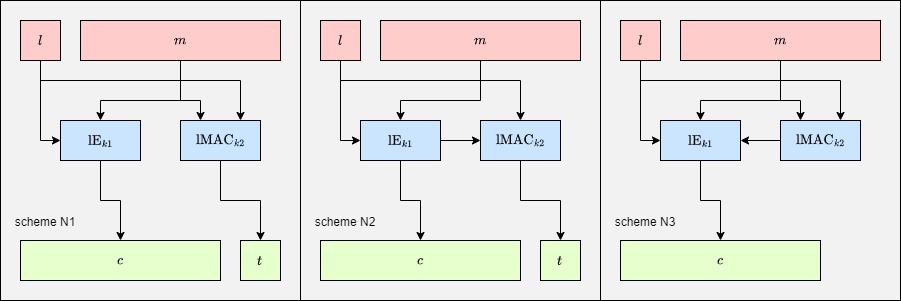
\includegraphics[scale = 0.4]{images/N-schemes.png}
\caption{Adjusted N schemes from \gcrec}
\end{figure}

\begin{figure}[H]
    \begin{pchstack}[boxed,center,space=0.5cm]
        \pseudocode[lnstart=-1,linenumbering,head={AE.enc$(\keyinstance,\lockinstance,\messageinstance)$}]{
            (\keyinstance{}1,\keyinstance{}2) \result \keyinstance \\
            \ciphertextinstance' \result \text{E.enc}(\keyinstance{}1,\lockinstance,\messageinstance) \\
            \taginstance \result \text{M.mac}(\keyinstance{}2,\lockinstance,\messageinstance) \\
            \ciphertextinstance \result (\ciphertextinstance',\taginstance)\\
            \pcreturn \ciphertextinstance
        }
        \pseudocode[lnstart=4,linenumbering,head={AE.dec$(\keyinstance,\lockinstance,\ciphertextinstance)$}]{
            (\keyinstance{}1,\keyinstance{}2) \result \keyinstance \\
            (\ciphertextinstance',\taginstance) \result \ciphertextinstance \\
            \messageinstance \result \text{E.dec}(\keyinstance{}1,\lockinstance,\ciphertextinstance') \\
            \taginstance' \result \text{M.mac}(\keyinstance{}2,\lockinstance,\messageinstance) \\
            \pcif \taginstance = \taginstance' : \pcreturn \messageinstance \\
            \pcelse : \pcreturn \invalid
        }
    \end{pchstack}
\caption{Calls based on N1}
\end{figure}

\begin{figure}[H]
    \begin{pchstack}[boxed,center,space=0.5cm]
        \pseudocode[lnstart=-1,linenumbering,head={AE.enc$(\keyinstance,\lockinstance,\messageinstance)$}]{
            (\keyinstance{}1,\keyinstance{}2) \result \keyinstance\\
            \ciphertextinstance' \result \text{E.enc}(\keyinstance{}1,\lockinstance,\messageinstance)\\
            \taginstance \result \text{M.mac}(\keyinstance{}2,\lockinstance,\ciphertextinstance')\\
            \ciphertextinstance \result (\ciphertextinstance',\taginstance)\\
            \pcreturn \ciphertextinstance
        }
        \pseudocode[lnstart=4,linenumbering,head={AE.dec$(\keyinstance,\lockinstance,\ciphertextinstance)$}]{
            (\keyinstance{}1,\keyinstance{}2) \result \keyinstance\\
            (\ciphertextinstance',\taginstance) \result \ciphertextinstance\\
            \messageinstance \result \text{E.dec}(\keyinstance{}1,\lockinstance,\ciphertextinstance')\\
            \taginstance' \result \text{M.mac}(\keyinstance{}2,\lockinstance,\ciphertextinstance')\\
            \pcif \taginstance = \taginstance' : \pcreturn \messageinstance \\
            \pcelse : \pcreturn \invalid
        }
    \end{pchstack}
\caption{Calls based on N2}
\end{figure}

\begin{figure}[H]
    \begin{pchstack}[boxed,center,space=0.5cm]
        \pseudocode[lnstart=-1,linenumbering,head={AE.enc$(\keyinstance,\lockinstance,\messageinstance)$}]{
            (\keyinstance{}1,\keyinstance{}2) \result \keyinstance\\
            \taginstance \result \text{M.mac}(\keyinstance{}2,\lockinstance,\messageinstance)\\
            \messageinstance' \result \messageinstance \concatinate \taginstance\\
            \ciphertextinstance \result E.enc(\keyinstance{}1,\lockinstance,\messageinstance')\\
            \pcreturn \ciphertextinstance
        }
        \pseudocode[lnstart=4,linenumbering,head={AE.dec$(\keyinstance,\lockinstance,\ciphertextinstance)$}]{
            (\keyinstance{}1,\keyinstance{}2) \result \keyinstance\\
            \messageinstance' \result \text{E.dec}(\keyinstance{}1,\lockinstance,\ciphertextinstance)\\
            (\messageinstance,\taginstance) \result \messageinstance'\\
            \taginstance' \result \text{M.mac}(\keyinstance{}2,\lockinstance,\messageinstance)\\
            \pcif \taginstance = \taginstance' : \pcreturn \messageinstance \\
            \pcelse : \pcreturn \invalid
        }
    \end{pchstack}
\caption{Calls based on N3}
\end{figure}

\noindent We define the constructions secure if there is a tight reduction from breaking the loAE-security
of the scheme to breaking the loDEM-security and the loMAC security of the underlying primitives.

\section{Use cases}
should consist of:
\begin{itemize}
	\item possible use cases
\end{itemize}

\section{Related Work}
\textbf{Location not final yet}

\section{Conclusion}

\newpage
\printbibliography[heading=bibintoc,title={References}]
\section{Appendix}

\end{document}

\NeedsTeXFormat{LaTeX2e}
\ProvidesPackage{rutitlepage}[2022/02/21 Mart Lubbers]
\RequirePackage{geometry,graphicx,ifpdf,keyval,iflang}
\def\@rutitleauthors{\@author}
\def\@rutitleauthorstext{Aut\IfLanguageName{dutch}{eu}{ho}r:}
\def\@rutitledate{\@date}
\def\@rutitleinst{Radboud Universit\IfLanguageName{dutch}{eit}{y} Nijmegen}
\def\@rutitletitle{\@title}
\def\@rutitlelayout{twentytwo}
\newif\if@rutitlecolour\@rutitlecolourfalse
\define@key{maketitleru}{authors}{\def\@rutitleauthors{#1}}
\define@key{maketitleru}{authorstext}{\def\@rutitleauthorstext{#1}}
\define@key{maketitleru}{colour}[true]{\@rutitlecolourtrue}
\define@key{maketitleru}{course}{\def\@rutitlecourse{#1}}
\define@key{maketitleru}{date}{\def\@rutitledate{#1}}
\define@key{maketitleru}{institution}{\def\@rutitleinst{#1}}
\define@key{maketitleru}{layout}{\def\@rutitlelayout{#1}}
\define@key{maketitleru}{nextpagenr}{\def\@rutitlenextpagenr{#1}}
\define@key{maketitleru}{others}{\def\@rutitleothers{#1}}
\define@key{maketitleru}{subtitle}{\def\@rutitlesubtitle{#1}}
\define@key{maketitleru}{title}{\def\@rutitletitle{#1}}
\newcommand*{\rutitlepage@printothers}[2]{\textit{#1}\\#2}
\newcommand*{\rutitlepage@sepothers}{\\[\baselineskip]}
\newcommand*{\rutitlepage@others}[2]{%
	\rutitlepage@printothers{#1}{#2}%
	\kernel@ifnextchar,{\rutitlepage@sepothers\rutitlepage@otherslist@}\relax}
\newcommand*{\rutitlepage@otherslist}[1]{%
	\expandafter\rutitlepage@others#1}
\def\rutitlepage@otherslist@,#1{\rutitlepage@otherslist{{#1}}}
\newcommand{\rutitle@layout@twentytwo}[0]{
	\newgeometry{left=25mm,top=25mm,right=15mm,bottom=10mm,hmarginratio=1:1}
	\begin{titlepage}%
		\null\vfill%
		\parindent0pt
		\ifdefined\@rutitlecourse\textsc{\LARGE\@rutitlecourse}\\[1.5cm]\fi
		{\Huge\bfseries\@rutitletitle}%
		\ifdefined\@rutitlesubtitle{\\[2\baselineskip]\large\itshape\@rutitlesubtitle\/}\fi\\[4\baselineskip]
		{\Large\scshape\@rutitleauthors}\\[\baselineskip]
		{\large\@rutitledate}
		\vfill

		\ifdefined\@rutitleothers\rutitlepage@otherslist\@rutitleothers\fi
		\vfill

		\hfill
		\ifpdf\includegraphics[width=80mm]{rutitlepage-logo-\IfLanguageName{dutch}{nl-}{}\if@rutitlecolour cmyk\else bw\fi.pdf}\\
		\else\includegraphics[width=80mm]{rutitlepage-logo-\IfLanguageName{dutch}{nl-}{}\if@rutitlecolour cmyk\else bw\fi.eps}\\
		\fi
	\end{titlepage}
	\restoregeometry%
}
\newcommand{\rutitle@layout@seventeen}[0]{
	\newgeometry{left=25mm,top=25mm,right=15mm,bottom=10mm,hmarginratio=1:1}
	\begin{titlepage}%
		\null\vfill%
		\parindent0pt
		{\Huge\bfseries\@rutitletitle}%
		\ifdefined\@rutitlesubtitle{\\[2\baselineskip]\large\itshape\@rutitlesubtitle\/}\fi\\[4\baselineskip]
		{\Large\scshape\@rutitleauthors}\\[\baselineskip]
		{\large\@rutitledate}
		\vfill

		\ifdefined\@rutitleothers\rutitlepage@otherslist\@rutitleothers\fi
		\vfill

		\hfill
		\ifpdf\includegraphics[width=80mm]{rutitlepage-logo-\IfLanguageName{dutch}{nl-}{}\if@rutitlecolour cmyk\else bw\fi.pdf}\\
		\else\includegraphics[width=80mm]{rutitlepage-logo-\IfLanguageName{dutch}{nl-}{}\if@rutitlecolour cmyk\else bw\fi.eps}\\
		\fi
	\end{titlepage}
	\restoregeometry%
}
\newcommand{\rutitle@layout@traditional}[0]{
	\newgeometry{hmarginratio=1:1}
	\begin{titlepage}
		\begin{center}
			\ifdefined\@rutitlecourse\textsc{\LARGE\@rutitlecourse}\\[1.5cm]\fi
			\ifpdf\includegraphics[height=150pt]{rutitlepage-logo.pdf}\\
			\else\includegraphics[height=150pt]{rutitlepage-logo.eps}\\
			\fi
			\vspace{0.4cm}
			\textsc{\Large\@rutitleinst}\\[1cm]
			\hrule
			\vspace{0.4cm}
			\textbf{\large\@rutitletitle}\\[0.4cm]
			\hrule
			\ifdefined\@rutitlesubtitle
				\vspace{0.4cm}
				\textit{\@rutitlesubtitle}\\[1cm]
			\else
				\vspace{2cm}
			\fi
			\begin{minipage}[t]{0.45\textwidth}
				\begin{flushleft}\large
					\textit{\@rutitleauthorstext}\\
					\@rutitleauthors{}
				\end{flushleft}
			\end{minipage}
			\begin{minipage}[t]{0.45\textwidth}
				\begin{flushright}\large
					\ifdefined\@rutitleothers
					\renewcommand{\rutitlepage@printothers}[2]{\textit{##1}\\##2}
					\renewcommand{\rutitlepage@sepothers}[0]{

						\vspace{8mm}}
					\rutitlepage@otherslist\@rutitleothers
					\fi
				\end{flushright}
			\end{minipage}
			\vfill
			{\large\@rutitledate}
		\end{center}
	\end{titlepage}
	\restoregeometry%
}
\newcommand{\maketitleru}[1][]{
	\setkeys{maketitleru}{#1}
	\ifcsname%
		rutitle@layout@\@rutitlelayout\endcsname
		\expandafter\csname rutitle@layout@\@rutitlelayout\endcsname
	\else
		\PackageError{rutitlepage}
			{Unknown layout `\@rutitlelayout'.}
			{The `layout' key of \maketitleru\space contained an unknown layout.\MessageBreak{}
			 Check the package documentation for the possible layouts.}
	\fi
	\ifdefined\@rutitlenextpagenr\setcounter{page}{\@rutitlenextpagenr}\fi%
}